\batchmode
\documentclass[twoside]{book}

% Packages required by doxygen
\usepackage{fixltx2e}
\usepackage{calc}
\usepackage{doxygen}
\usepackage[export]{adjustbox} % also loads graphicx
\usepackage{graphicx}
\usepackage[utf8]{inputenc}
\usepackage{makeidx}
\usepackage{multicol}
\usepackage{multirow}
\PassOptionsToPackage{warn}{textcomp}
\usepackage{textcomp}
\usepackage[nointegrals]{wasysym}
\usepackage[table]{xcolor}

% Font selection
\usepackage[T1]{fontenc}
\usepackage[scaled=.90]{helvet}
\usepackage{courier}
\usepackage{amssymb}
\usepackage{sectsty}
\renewcommand{\familydefault}{\sfdefault}
\allsectionsfont{%
  \fontseries{bc}\selectfont%
  \color{darkgray}%
}
\renewcommand{\DoxyLabelFont}{%
  \fontseries{bc}\selectfont%
  \color{darkgray}%
}
\newcommand{\+}{\discretionary{\mbox{\scriptsize$\hookleftarrow$}}{}{}}

% Page & text layout
\usepackage{geometry}
\geometry{%
  a4paper,%
  top=2.5cm,%
  bottom=2.5cm,%
  left=2.5cm,%
  right=2.5cm%
}
\tolerance=750
\hfuzz=15pt
\hbadness=750
\setlength{\emergencystretch}{15pt}
\setlength{\parindent}{0cm}
\setlength{\parskip}{3ex plus 2ex minus 2ex}
\makeatletter
\renewcommand{\paragraph}{%
  \@startsection{paragraph}{4}{0ex}{-1.0ex}{1.0ex}{%
    \normalfont\normalsize\bfseries\SS@parafont%
  }%
}
\renewcommand{\subparagraph}{%
  \@startsection{subparagraph}{5}{0ex}{-1.0ex}{1.0ex}{%
    \normalfont\normalsize\bfseries\SS@subparafont%
  }%
}
\makeatother

% Headers & footers
\usepackage{fancyhdr}
\pagestyle{fancyplain}
\fancyhead[LE]{\fancyplain{}{\bfseries\thepage}}
\fancyhead[CE]{\fancyplain{}{}}
\fancyhead[RE]{\fancyplain{}{\bfseries\leftmark}}
\fancyhead[LO]{\fancyplain{}{\bfseries\rightmark}}
\fancyhead[CO]{\fancyplain{}{}}
\fancyhead[RO]{\fancyplain{}{\bfseries\thepage}}
\fancyfoot[LE]{\fancyplain{}{}}
\fancyfoot[CE]{\fancyplain{}{}}
\fancyfoot[RE]{\fancyplain{}{\bfseries\scriptsize Generated by Doxygen }}
\fancyfoot[LO]{\fancyplain{}{\bfseries\scriptsize Generated by Doxygen }}
\fancyfoot[CO]{\fancyplain{}{}}
\fancyfoot[RO]{\fancyplain{}{}}
\renewcommand{\footrulewidth}{0.4pt}
\renewcommand{\chaptermark}[1]{%
  \markboth{#1}{}%
}
\renewcommand{\sectionmark}[1]{%
  \markright{\thesection\ #1}%
}

% Indices & bibliography
\usepackage{natbib}
\usepackage[titles]{tocloft}
\setcounter{tocdepth}{3}
\setcounter{secnumdepth}{5}
\makeindex

% Hyperlinks (required, but should be loaded last)
\usepackage{ifpdf}
\ifpdf
  \usepackage[pdftex,pagebackref=true]{hyperref}
\else
  \usepackage[ps2pdf,pagebackref=true]{hyperref}
\fi
\hypersetup{%
  colorlinks=true,%
  linkcolor=blue,%
  citecolor=blue,%
  unicode%
}

% Custom commands
\newcommand{\clearemptydoublepage}{%
  \newpage{\pagestyle{empty}\cleardoublepage}%
}

\usepackage{caption}
\captionsetup{labelsep=space,justification=centering,font={bf},singlelinecheck=off,skip=4pt,position=top}

%===== C O N T E N T S =====

\begin{document}

% Titlepage & ToC
\hypersetup{pageanchor=false,
             bookmarksnumbered=true
            }
\pagenumbering{alph}
\pagenumbering{arabic}
\hypersetup{pageanchor=true}

%--- Begin generated contents ---
\chapter{Example problem\+: Adaptive solution of the 3D Poisson equation in a spherical domain}
\label{index}\hypertarget{index}{}\hypertarget{index_q}{}\section{A few quick questions...}\label{index_q}
Since {\ttfamily oomph-\/lib} is developed as open-\/source software, any evidence that the code is being downloaded and used is very helpful for us as it helps to justify our continued work on this project.

We would therefore be extremely grateful if you could provide the information requested in the form below. Pressing the \char`\"{}submit\char`\"{} button will get you to the actual download page.

{\bfseries Note\+:} 
\begin{DoxyItemize}
\item All information will be treated as confidential. 
\item If you provide your email address and check the appropriate box we will add you to our mailing list to inform you of upgrades and bug fixes to the code. Rest assured that the mailing list is {\bfseries very low volume} -- we have better things to do than to bombard you with email. 
\item If you still feel reluctant to provide any of the information requested, feel free to enter some dummy input. The form will check that {\bfseries some} information has been entered but entering your name as \char`\"{}\+Joe Cool\char`\"{} is perfectly acceptable -- this is to discourage people from not providing the information simply because they are too lazy to type... 
\end{DoxyItemize}



 







 

 \hypertarget{index_pdf}{}\section{P\+D\+F file}\label{index_pdf}
A \href{../latex/refman.pdf}{\tt pdf version} of this document is available. \end{document}

\chapter{Namespace Index}
\section{Namespace List}
Here is a list of all namespaces with brief descriptions\+:\begin{DoxyCompactList}
\item\contentsline{section}{\hyperlink{namespaceGlobal__Physical__Variables}{Global\+\_\+\+Physical\+\_\+\+Variables} \\*Global variables that represent physical properties }{\pageref{namespaceGlobal__Physical__Variables}}{}
\item\contentsline{section}{\hyperlink{namespaceoomph}{oomph} }{\pageref{namespaceoomph}}{}
\item\contentsline{section}{\hyperlink{namespacePhysical__Variables}{Physical\+\_\+\+Variables} \\*Namespace for the solution of 2D linear shell equation }{\pageref{namespacePhysical__Variables}}{}
\end{DoxyCompactList}

\chapter{Hierarchical Index}
\section{Class Hierarchy}
This inheritance list is sorted roughly, but not completely, alphabetically\+:\begin{DoxyCompactList}
\item Problem\begin{DoxyCompactList}
\item \contentsline{section}{Unstructured\+Solid\+Problem$<$ E\+L\+E\+M\+E\+NT $>$}{\pageref{classUnstructuredSolidProblem}}{}
\end{DoxyCompactList}
\end{DoxyCompactList}

\chapter{Class Index}
\section{Class List}
Here are the classes, structs, unions and interfaces with brief descriptions\+:\begin{DoxyCompactList}
\item\contentsline{section}{\hyperlink{classPMLProblem}{P\+M\+L\+Problem$<$ E\+L\+E\+M\+E\+N\+T $>$} }{\pageref{classPMLProblem}}{}
\item\contentsline{section}{\hyperlink{classGlobalParameters_1_1TestPMLMapping}{Global\+Parameters\+::\+Test\+P\+M\+L\+Mapping} }{\pageref{classGlobalParameters_1_1TestPMLMapping}}{}
\end{DoxyCompactList}

\chapter{File Index}
\section{File List}
Here is a list of all files with brief descriptions\+:\begin{DoxyCompactList}
\item\contentsline{section}{\hyperlink{jeffery__orbit_8cc}{jeffery\+\_\+orbit.\+cc} }{\pageref{jeffery__orbit_8cc}}{}
\item\contentsline{section}{\hyperlink{jeffery__orbit_8txt__doxygenified_8h}{jeffery\+\_\+orbit.\+txt\+\_\+doxygenified.\+h} }{\pageref{jeffery__orbit_8txt__doxygenified_8h}}{}
\item\contentsline{section}{\hyperlink{my__taylor__hood__elements_8h}{my\+\_\+taylor\+\_\+hood\+\_\+elements.\+h} }{\pageref{my__taylor__hood__elements_8h}}{}
\end{DoxyCompactList}

\chapter{Namespace Documentation}
\hypertarget{namespaceTanhSolnForPoisson}{}\section{Tanh\+Soln\+For\+Poisson Namespace Reference}
\label{namespaceTanhSolnForPoisson}\index{Tanh\+Soln\+For\+Poisson@{Tanh\+Soln\+For\+Poisson}}


Namespace for exact solution for Poisson equation with sharp step.  


\subsection*{Functions}
\begin{DoxyCompactItemize}
\item 
void \hyperlink{namespaceTanhSolnForPoisson_af7896e9c18ce6438c73ae2a875e8b7de}{get\+\_\+exact\+\_\+u} (const Vector$<$ double $>$ \&x, Vector$<$ double $>$ \&u)
\begin{DoxyCompactList}\small\item\em Exact solution as a Vector. \end{DoxyCompactList}\item 
void \hyperlink{namespaceTanhSolnForPoisson_af197decab980d38d2037032780723984}{get\+\_\+exact\+\_\+u} (const Vector$<$ double $>$ \&x, double \&u)
\begin{DoxyCompactList}\small\item\em Exact solution as a scalar. \end{DoxyCompactList}\item 
void \hyperlink{namespaceTanhSolnForPoisson_ae1b9d6789ff301e3d63a4e292213036c}{get\+\_\+source} (const Vector$<$ double $>$ \&x, double \&source)
\begin{DoxyCompactList}\small\item\em Source function to make it an exact solution. \end{DoxyCompactList}\end{DoxyCompactItemize}
\subsection*{Variables}
\begin{DoxyCompactItemize}
\item 
double \hyperlink{namespaceTanhSolnForPoisson_ae676ccd186d5df119cce811596d949c1}{Alpha}
\begin{DoxyCompactList}\small\item\em Parameter for steepness of step. \end{DoxyCompactList}\item 
double \hyperlink{namespaceTanhSolnForPoisson_ae07364a1d73b28e5e250bda6c8954f01}{Beta}
\begin{DoxyCompactList}\small\item\em Parameter for angle of step. \end{DoxyCompactList}\end{DoxyCompactItemize}


\subsection{Detailed Description}
Namespace for exact solution for Poisson equation with sharp step. 

\subsection{Function Documentation}
\mbox{\Hypertarget{namespaceTanhSolnForPoisson_af7896e9c18ce6438c73ae2a875e8b7de}\label{namespaceTanhSolnForPoisson_af7896e9c18ce6438c73ae2a875e8b7de}} 
\index{Tanh\+Soln\+For\+Poisson@{Tanh\+Soln\+For\+Poisson}!get\+\_\+exact\+\_\+u@{get\+\_\+exact\+\_\+u}}
\index{get\+\_\+exact\+\_\+u@{get\+\_\+exact\+\_\+u}!Tanh\+Soln\+For\+Poisson@{Tanh\+Soln\+For\+Poisson}}
\subsubsection{\texorpdfstring{get\+\_\+exact\+\_\+u()}{get\_exact\_u()}\hspace{0.1cm}{\footnotesize\ttfamily [1/2]}}
{\footnotesize\ttfamily void Tanh\+Soln\+For\+Poisson\+::get\+\_\+exact\+\_\+u (\begin{DoxyParamCaption}\item[{const Vector$<$ double $>$ \&}]{x,  }\item[{Vector$<$ double $>$ \&}]{u }\end{DoxyParamCaption})}



Exact solution as a Vector. 



Definition at line 61 of file mesh\+\_\+from\+\_\+triangle\+\_\+poisson.\+cc.



Referenced by Poisson\+Problem$<$ E\+L\+E\+M\+E\+N\+T $>$\+::actions\+\_\+before\+\_\+newton\+\_\+solve(), and Poisson\+Problem$<$ E\+L\+E\+M\+E\+N\+T $>$\+::doc\+\_\+solution().

\mbox{\Hypertarget{namespaceTanhSolnForPoisson_af197decab980d38d2037032780723984}\label{namespaceTanhSolnForPoisson_af197decab980d38d2037032780723984}} 
\index{Tanh\+Soln\+For\+Poisson@{Tanh\+Soln\+For\+Poisson}!get\+\_\+exact\+\_\+u@{get\+\_\+exact\+\_\+u}}
\index{get\+\_\+exact\+\_\+u@{get\+\_\+exact\+\_\+u}!Tanh\+Soln\+For\+Poisson@{Tanh\+Soln\+For\+Poisson}}
\subsubsection{\texorpdfstring{get\+\_\+exact\+\_\+u()}{get\_exact\_u()}\hspace{0.1cm}{\footnotesize\ttfamily [2/2]}}
{\footnotesize\ttfamily void Tanh\+Soln\+For\+Poisson\+::get\+\_\+exact\+\_\+u (\begin{DoxyParamCaption}\item[{const Vector$<$ double $>$ \&}]{x,  }\item[{double \&}]{u }\end{DoxyParamCaption})}



Exact solution as a scalar. 



Definition at line 68 of file mesh\+\_\+from\+\_\+triangle\+\_\+poisson.\+cc.

\mbox{\Hypertarget{namespaceTanhSolnForPoisson_ae1b9d6789ff301e3d63a4e292213036c}\label{namespaceTanhSolnForPoisson_ae1b9d6789ff301e3d63a4e292213036c}} 
\index{Tanh\+Soln\+For\+Poisson@{Tanh\+Soln\+For\+Poisson}!get\+\_\+source@{get\+\_\+source}}
\index{get\+\_\+source@{get\+\_\+source}!Tanh\+Soln\+For\+Poisson@{Tanh\+Soln\+For\+Poisson}}
\subsubsection{\texorpdfstring{get\+\_\+source()}{get\_source()}}
{\footnotesize\ttfamily void Tanh\+Soln\+For\+Poisson\+::get\+\_\+source (\begin{DoxyParamCaption}\item[{const Vector$<$ double $>$ \&}]{x,  }\item[{double \&}]{source }\end{DoxyParamCaption})}



Source function to make it an exact solution. 



Definition at line 75 of file mesh\+\_\+from\+\_\+triangle\+\_\+poisson.\+cc.



Referenced by main().



\subsection{Variable Documentation}
\mbox{\Hypertarget{namespaceTanhSolnForPoisson_ae676ccd186d5df119cce811596d949c1}\label{namespaceTanhSolnForPoisson_ae676ccd186d5df119cce811596d949c1}} 
\index{Tanh\+Soln\+For\+Poisson@{Tanh\+Soln\+For\+Poisson}!Alpha@{Alpha}}
\index{Alpha@{Alpha}!Tanh\+Soln\+For\+Poisson@{Tanh\+Soln\+For\+Poisson}}
\subsubsection{\texorpdfstring{Alpha}{Alpha}}
{\footnotesize\ttfamily double Tanh\+Soln\+For\+Poisson\+::\+Alpha}



Parameter for steepness of step. 



Definition at line 54 of file mesh\+\_\+from\+\_\+triangle\+\_\+poisson.\+cc.



Referenced by Poisson\+Problem$<$ E\+L\+E\+M\+E\+N\+T $>$\+::\+Poisson\+Problem().

\mbox{\Hypertarget{namespaceTanhSolnForPoisson_ae07364a1d73b28e5e250bda6c8954f01}\label{namespaceTanhSolnForPoisson_ae07364a1d73b28e5e250bda6c8954f01}} 
\index{Tanh\+Soln\+For\+Poisson@{Tanh\+Soln\+For\+Poisson}!Beta@{Beta}}
\index{Beta@{Beta}!Tanh\+Soln\+For\+Poisson@{Tanh\+Soln\+For\+Poisson}}
\subsubsection{\texorpdfstring{Beta}{Beta}}
{\footnotesize\ttfamily double Tanh\+Soln\+For\+Poisson\+::\+Beta}



Parameter for angle of step. 



Definition at line 57 of file mesh\+\_\+from\+\_\+triangle\+\_\+poisson.\+cc.



Referenced by Poisson\+Problem$<$ E\+L\+E\+M\+E\+N\+T $>$\+::\+Poisson\+Problem().


\chapter{Class Documentation}
\hypertarget{classEighthSpherePoissonProblem}{}\section{Eighth\+Sphere\+Poisson\+Problem$<$ E\+L\+E\+M\+E\+NT $>$ Class Template Reference}
\label{classEighthSpherePoissonProblem}\index{Eighth\+Sphere\+Poisson\+Problem$<$ E\+L\+E\+M\+E\+N\+T $>$@{Eighth\+Sphere\+Poisson\+Problem$<$ E\+L\+E\+M\+E\+N\+T $>$}}


Poisson problem in refineable eighth of a sphere mesh.  


Inheritance diagram for Eighth\+Sphere\+Poisson\+Problem$<$ E\+L\+E\+M\+E\+NT $>$\+:\begin{figure}[H]
\begin{center}
\leavevmode
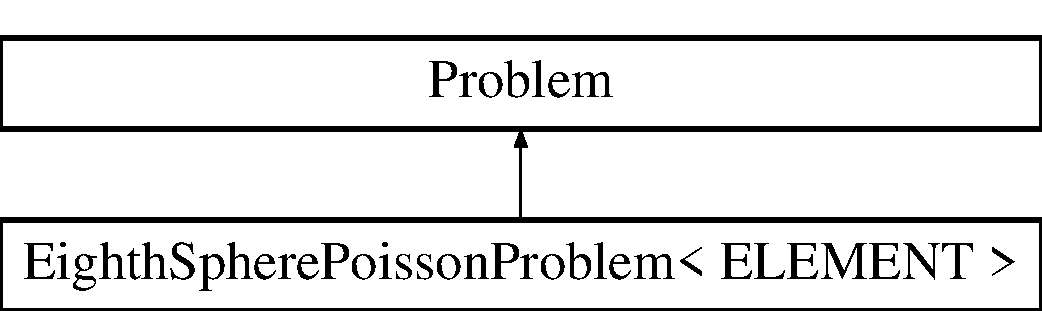
\includegraphics[height=2.000000cm]{classEighthSpherePoissonProblem}
\end{center}
\end{figure}
\subsection*{Public Member Functions}
\begin{DoxyCompactItemize}
\item 
\hyperlink{classEighthSpherePoissonProblem_ae51db2c3e80f0d5628e4d81eb1c11db4}{Eighth\+Sphere\+Poisson\+Problem} (Poisson\+Equations$<$ 3 $>$\+::Poisson\+Source\+Fct\+Pt source\+\_\+fct\+\_\+pt)
\begin{DoxyCompactList}\small\item\em Constructor\+: Pass pointer to source function. \end{DoxyCompactList}\item 
\hyperlink{classEighthSpherePoissonProblem_a043c7aa08c939fdc019870ad2c2270cc}{$\sim$\+Eighth\+Sphere\+Poisson\+Problem} ()
\begin{DoxyCompactList}\small\item\em Destructor\+: Empty. \end{DoxyCompactList}\item 
Refineable\+Eighth\+Sphere\+Mesh$<$ E\+L\+E\+M\+E\+NT $>$ $\ast$ \hyperlink{classEighthSpherePoissonProblem_aa33edbb75ba8fe8d4daac3c940a7ff6a}{mesh\+\_\+pt} ()
\begin{DoxyCompactList}\small\item\em Overload generic access function by one that returns a pointer to the specific mesh. \end{DoxyCompactList}\item 
void \hyperlink{classEighthSpherePoissonProblem_a480189fe5d2f42fe3ff6062d5f151ea3}{actions\+\_\+after\+\_\+newton\+\_\+solve} ()
\begin{DoxyCompactList}\small\item\em Update the problem specs after solve (empty) \end{DoxyCompactList}\item 
void \hyperlink{classEighthSpherePoissonProblem_af82dd7abdf631950a68c997af314be5d}{actions\+\_\+before\+\_\+newton\+\_\+solve} ()
\begin{DoxyCompactList}\small\item\em Update the problem specs before solve\+: Set Dirchlet boundary conditions from exact solution. \end{DoxyCompactList}\item 
void \hyperlink{classEighthSpherePoissonProblem_ac8e9911536d04bab829cfe92bb40e302}{doc\+\_\+solution} (Doc\+Info \&doc\+\_\+info)
\begin{DoxyCompactList}\small\item\em Doc the solution. \end{DoxyCompactList}\end{DoxyCompactItemize}
\subsection*{Private Attributes}
\begin{DoxyCompactItemize}
\item 
Poisson\+Equations$<$ 3 $>$\+::Poisson\+Source\+Fct\+Pt \hyperlink{classEighthSpherePoissonProblem_af41ed0ce372d5932c64b3cd4fe69f312}{Source\+\_\+fct\+\_\+pt}
\begin{DoxyCompactList}\small\item\em Pointer to source function. \end{DoxyCompactList}\end{DoxyCompactItemize}


\subsection{Detailed Description}
\subsubsection*{template$<$class E\+L\+E\+M\+E\+NT$>$\newline
class Eighth\+Sphere\+Poisson\+Problem$<$ E\+L\+E\+M\+E\+N\+T $>$}

Poisson problem in refineable eighth of a sphere mesh. 

Definition at line 135 of file eighth\+\_\+sphere\+\_\+poisson.\+cc.



\subsection{Constructor \& Destructor Documentation}
\mbox{\Hypertarget{classEighthSpherePoissonProblem_ae51db2c3e80f0d5628e4d81eb1c11db4}\label{classEighthSpherePoissonProblem_ae51db2c3e80f0d5628e4d81eb1c11db4}} 
\index{Eighth\+Sphere\+Poisson\+Problem@{Eighth\+Sphere\+Poisson\+Problem}!Eighth\+Sphere\+Poisson\+Problem@{Eighth\+Sphere\+Poisson\+Problem}}
\index{Eighth\+Sphere\+Poisson\+Problem@{Eighth\+Sphere\+Poisson\+Problem}!Eighth\+Sphere\+Poisson\+Problem@{Eighth\+Sphere\+Poisson\+Problem}}
\subsubsection{\texorpdfstring{Eighth\+Sphere\+Poisson\+Problem()}{EighthSpherePoissonProblem()}}
{\footnotesize\ttfamily template$<$class E\+L\+E\+M\+E\+NT $>$ \\
\hyperlink{classEighthSpherePoissonProblem}{Eighth\+Sphere\+Poisson\+Problem}$<$ E\+L\+E\+M\+E\+NT $>$\+::\hyperlink{classEighthSpherePoissonProblem}{Eighth\+Sphere\+Poisson\+Problem} (\begin{DoxyParamCaption}\item[{Poisson\+Equations$<$ 3 $>$\+::Poisson\+Source\+Fct\+Pt}]{source\+\_\+fct\+\_\+pt }\end{DoxyParamCaption})}



Constructor\+: Pass pointer to source function. 

Constructor for Poisson problem on eighth of a sphere mesh. Create mesh for sphere of radius 5 

Definition at line 199 of file eighth\+\_\+sphere\+\_\+poisson.\+cc.



References Tanh\+Soln\+For\+Poisson\+::\+Alpha, Eighth\+Sphere\+Poisson\+Problem$<$ E\+L\+E\+M\+E\+N\+T $>$\+::mesh\+\_\+pt(), and Eighth\+Sphere\+Poisson\+Problem$<$ E\+L\+E\+M\+E\+N\+T $>$\+::\+Source\+\_\+fct\+\_\+pt.

\mbox{\Hypertarget{classEighthSpherePoissonProblem_a043c7aa08c939fdc019870ad2c2270cc}\label{classEighthSpherePoissonProblem_a043c7aa08c939fdc019870ad2c2270cc}} 
\index{Eighth\+Sphere\+Poisson\+Problem@{Eighth\+Sphere\+Poisson\+Problem}!````~Eighth\+Sphere\+Poisson\+Problem@{$\sim$\+Eighth\+Sphere\+Poisson\+Problem}}
\index{````~Eighth\+Sphere\+Poisson\+Problem@{$\sim$\+Eighth\+Sphere\+Poisson\+Problem}!Eighth\+Sphere\+Poisson\+Problem@{Eighth\+Sphere\+Poisson\+Problem}}
\subsubsection{\texorpdfstring{$\sim$\+Eighth\+Sphere\+Poisson\+Problem()}{~EighthSpherePoissonProblem()}}
{\footnotesize\ttfamily template$<$class E\+L\+E\+M\+E\+NT$>$ \\
\hyperlink{classEighthSpherePoissonProblem}{Eighth\+Sphere\+Poisson\+Problem}$<$ E\+L\+E\+M\+E\+NT $>$\+::$\sim$\hyperlink{classEighthSpherePoissonProblem}{Eighth\+Sphere\+Poisson\+Problem} (\begin{DoxyParamCaption}{ }\end{DoxyParamCaption})\hspace{0.3cm}{\ttfamily [inline]}}



Destructor\+: Empty. 



Definition at line 145 of file eighth\+\_\+sphere\+\_\+poisson.\+cc.



\subsection{Member Function Documentation}
\mbox{\Hypertarget{classEighthSpherePoissonProblem_a480189fe5d2f42fe3ff6062d5f151ea3}\label{classEighthSpherePoissonProblem_a480189fe5d2f42fe3ff6062d5f151ea3}} 
\index{Eighth\+Sphere\+Poisson\+Problem@{Eighth\+Sphere\+Poisson\+Problem}!actions\+\_\+after\+\_\+newton\+\_\+solve@{actions\+\_\+after\+\_\+newton\+\_\+solve}}
\index{actions\+\_\+after\+\_\+newton\+\_\+solve@{actions\+\_\+after\+\_\+newton\+\_\+solve}!Eighth\+Sphere\+Poisson\+Problem@{Eighth\+Sphere\+Poisson\+Problem}}
\subsubsection{\texorpdfstring{actions\+\_\+after\+\_\+newton\+\_\+solve()}{actions\_after\_newton\_solve()}}
{\footnotesize\ttfamily template$<$class E\+L\+E\+M\+E\+NT$>$ \\
void \hyperlink{classEighthSpherePoissonProblem}{Eighth\+Sphere\+Poisson\+Problem}$<$ E\+L\+E\+M\+E\+NT $>$\+::actions\+\_\+after\+\_\+newton\+\_\+solve (\begin{DoxyParamCaption}{ }\end{DoxyParamCaption})\hspace{0.3cm}{\ttfamily [inline]}}



Update the problem specs after solve (empty) 



Definition at line 155 of file eighth\+\_\+sphere\+\_\+poisson.\+cc.

\mbox{\Hypertarget{classEighthSpherePoissonProblem_af82dd7abdf631950a68c997af314be5d}\label{classEighthSpherePoissonProblem_af82dd7abdf631950a68c997af314be5d}} 
\index{Eighth\+Sphere\+Poisson\+Problem@{Eighth\+Sphere\+Poisson\+Problem}!actions\+\_\+before\+\_\+newton\+\_\+solve@{actions\+\_\+before\+\_\+newton\+\_\+solve}}
\index{actions\+\_\+before\+\_\+newton\+\_\+solve@{actions\+\_\+before\+\_\+newton\+\_\+solve}!Eighth\+Sphere\+Poisson\+Problem@{Eighth\+Sphere\+Poisson\+Problem}}
\subsubsection{\texorpdfstring{actions\+\_\+before\+\_\+newton\+\_\+solve()}{actions\_before\_newton\_solve()}}
{\footnotesize\ttfamily template$<$class E\+L\+E\+M\+E\+NT$>$ \\
void \hyperlink{classEighthSpherePoissonProblem}{Eighth\+Sphere\+Poisson\+Problem}$<$ E\+L\+E\+M\+E\+NT $>$\+::actions\+\_\+before\+\_\+newton\+\_\+solve (\begin{DoxyParamCaption}{ }\end{DoxyParamCaption})\hspace{0.3cm}{\ttfamily [inline]}}



Update the problem specs before solve\+: Set Dirchlet boundary conditions from exact solution. 



Definition at line 159 of file eighth\+\_\+sphere\+\_\+poisson.\+cc.



References Tanh\+Soln\+For\+Poisson\+::get\+\_\+exact\+\_\+u().

\mbox{\Hypertarget{classEighthSpherePoissonProblem_ac8e9911536d04bab829cfe92bb40e302}\label{classEighthSpherePoissonProblem_ac8e9911536d04bab829cfe92bb40e302}} 
\index{Eighth\+Sphere\+Poisson\+Problem@{Eighth\+Sphere\+Poisson\+Problem}!doc\+\_\+solution@{doc\+\_\+solution}}
\index{doc\+\_\+solution@{doc\+\_\+solution}!Eighth\+Sphere\+Poisson\+Problem@{Eighth\+Sphere\+Poisson\+Problem}}
\subsubsection{\texorpdfstring{doc\+\_\+solution()}{doc\_solution()}}
{\footnotesize\ttfamily template$<$class E\+L\+E\+M\+E\+NT $>$ \\
void \hyperlink{classEighthSpherePoissonProblem}{Eighth\+Sphere\+Poisson\+Problem}$<$ E\+L\+E\+M\+E\+NT $>$\+::doc\+\_\+solution (\begin{DoxyParamCaption}\item[{Doc\+Info \&}]{doc\+\_\+info }\end{DoxyParamCaption})}



Doc the solution. 



Definition at line 275 of file eighth\+\_\+sphere\+\_\+poisson.\+cc.



References Tanh\+Soln\+For\+Poisson\+::get\+\_\+exact\+\_\+u(), and Eighth\+Sphere\+Poisson\+Problem$<$ E\+L\+E\+M\+E\+N\+T $>$\+::mesh\+\_\+pt().



Referenced by main().

\mbox{\Hypertarget{classEighthSpherePoissonProblem_aa33edbb75ba8fe8d4daac3c940a7ff6a}\label{classEighthSpherePoissonProblem_aa33edbb75ba8fe8d4daac3c940a7ff6a}} 
\index{Eighth\+Sphere\+Poisson\+Problem@{Eighth\+Sphere\+Poisson\+Problem}!mesh\+\_\+pt@{mesh\+\_\+pt}}
\index{mesh\+\_\+pt@{mesh\+\_\+pt}!Eighth\+Sphere\+Poisson\+Problem@{Eighth\+Sphere\+Poisson\+Problem}}
\subsubsection{\texorpdfstring{mesh\+\_\+pt()}{mesh\_pt()}}
{\footnotesize\ttfamily template$<$class E\+L\+E\+M\+E\+NT$>$ \\
Refineable\+Eighth\+Sphere\+Mesh$<$E\+L\+E\+M\+E\+NT$>$$\ast$ \hyperlink{classEighthSpherePoissonProblem}{Eighth\+Sphere\+Poisson\+Problem}$<$ E\+L\+E\+M\+E\+NT $>$\+::mesh\+\_\+pt (\begin{DoxyParamCaption}{ }\end{DoxyParamCaption})\hspace{0.3cm}{\ttfamily [inline]}}



Overload generic access function by one that returns a pointer to the specific mesh. 



Definition at line 149 of file eighth\+\_\+sphere\+\_\+poisson.\+cc.



Referenced by Eighth\+Sphere\+Poisson\+Problem$<$ E\+L\+E\+M\+E\+N\+T $>$\+::doc\+\_\+solution(), Eighth\+Sphere\+Poisson\+Problem$<$ E\+L\+E\+M\+E\+N\+T $>$\+::\+Eighth\+Sphere\+Poisson\+Problem(), and main().



\subsection{Member Data Documentation}
\mbox{\Hypertarget{classEighthSpherePoissonProblem_af41ed0ce372d5932c64b3cd4fe69f312}\label{classEighthSpherePoissonProblem_af41ed0ce372d5932c64b3cd4fe69f312}} 
\index{Eighth\+Sphere\+Poisson\+Problem@{Eighth\+Sphere\+Poisson\+Problem}!Source\+\_\+fct\+\_\+pt@{Source\+\_\+fct\+\_\+pt}}
\index{Source\+\_\+fct\+\_\+pt@{Source\+\_\+fct\+\_\+pt}!Eighth\+Sphere\+Poisson\+Problem@{Eighth\+Sphere\+Poisson\+Problem}}
\subsubsection{\texorpdfstring{Source\+\_\+fct\+\_\+pt}{Source\_fct\_pt}}
{\footnotesize\ttfamily template$<$class E\+L\+E\+M\+E\+NT$>$ \\
Poisson\+Equations$<$3$>$\+::Poisson\+Source\+Fct\+Pt \hyperlink{classEighthSpherePoissonProblem}{Eighth\+Sphere\+Poisson\+Problem}$<$ E\+L\+E\+M\+E\+NT $>$\+::Source\+\_\+fct\+\_\+pt\hspace{0.3cm}{\ttfamily [private]}}



Pointer to source function. 



Definition at line 187 of file eighth\+\_\+sphere\+\_\+poisson.\+cc.



Referenced by Eighth\+Sphere\+Poisson\+Problem$<$ E\+L\+E\+M\+E\+N\+T $>$\+::\+Eighth\+Sphere\+Poisson\+Problem().



The documentation for this class was generated from the following file\+:\begin{DoxyCompactItemize}
\item 
\hyperlink{eighth__sphere__poisson_8cc}{eighth\+\_\+sphere\+\_\+poisson.\+cc}\end{DoxyCompactItemize}

\chapter{File Documentation}
\hypertarget{eighth__sphere__poisson_8cc}{}\section{eighth\+\_\+sphere\+\_\+poisson.\+cc File Reference}
\label{eighth__sphere__poisson_8cc}\index{eighth\+\_\+sphere\+\_\+poisson.\+cc@{eighth\+\_\+sphere\+\_\+poisson.\+cc}}
\subsection*{Classes}
\begin{DoxyCompactItemize}
\item 
class \hyperlink{classEighthSpherePoissonProblem}{Eighth\+Sphere\+Poisson\+Problem$<$ E\+L\+E\+M\+E\+N\+T $>$}
\begin{DoxyCompactList}\small\item\em Poisson problem in refineable eighth of a sphere mesh. \end{DoxyCompactList}\end{DoxyCompactItemize}
\subsection*{Namespaces}
\begin{DoxyCompactItemize}
\item 
 \hyperlink{namespaceTanhSolnForPoisson}{Tanh\+Soln\+For\+Poisson}
\begin{DoxyCompactList}\small\item\em Namespace for exact solution for Poisson equation with sharp step. \end{DoxyCompactList}\end{DoxyCompactItemize}
\subsection*{Functions}
\begin{DoxyCompactItemize}
\item 
void \hyperlink{namespaceTanhSolnForPoisson_af7896e9c18ce6438c73ae2a875e8b7de}{Tanh\+Soln\+For\+Poisson\+::get\+\_\+exact\+\_\+u} (const Vector$<$ double $>$ \&x, Vector$<$ double $>$ \&u)
\item 
void \hyperlink{namespaceTanhSolnForPoisson_af197decab980d38d2037032780723984}{Tanh\+Soln\+For\+Poisson\+::get\+\_\+exact\+\_\+u} (const Vector$<$ double $>$ \&x, double \&u)
\begin{DoxyCompactList}\small\item\em Exact solution as a scalar. \end{DoxyCompactList}\item 
void \hyperlink{namespaceTanhSolnForPoisson_ae1b9d6789ff301e3d63a4e292213036c}{Tanh\+Soln\+For\+Poisson\+::get\+\_\+source} (const Vector$<$ double $>$ \&x, double \&source)
\begin{DoxyCompactList}\small\item\em Source function to make it an exact solution. \end{DoxyCompactList}\item 
int \hyperlink{eighth__sphere__poisson_8cc_a0ddf1224851353fc92bfbff6f499fa97}{main} (int argc, char $\ast$argv\mbox{[}$\,$\mbox{]})
\end{DoxyCompactItemize}
\subsection*{Variables}
\begin{DoxyCompactItemize}
\item 
double \hyperlink{namespaceTanhSolnForPoisson_ae676ccd186d5df119cce811596d949c1}{Tanh\+Soln\+For\+Poisson\+::\+Alpha} =1
\begin{DoxyCompactList}\small\item\em Parameter for steepness of step. \end{DoxyCompactList}\item 
double \hyperlink{namespaceTanhSolnForPoisson_ac3d25f0791c1363f487600e02757bc97}{Tanh\+Soln\+For\+Poisson\+::\+N\+\_\+x} =-\/1.\+0
\begin{DoxyCompactList}\small\item\em Orientation (non-\/normalised x-\/component of unit vector in direction of step plane) \end{DoxyCompactList}\item 
double \hyperlink{namespaceTanhSolnForPoisson_a482d668ef91071985d1f4ce7cf29a926}{Tanh\+Soln\+For\+Poisson\+::\+N\+\_\+y} =-\/1.\+0
\begin{DoxyCompactList}\small\item\em Orientation (non-\/normalised y-\/component of unit vector in direction of step plane) \end{DoxyCompactList}\item 
double \hyperlink{namespaceTanhSolnForPoisson_ae6b5b5d21747a45776004756dc97dc5c}{Tanh\+Soln\+For\+Poisson\+::\+N\+\_\+z} =1.\+0
\begin{DoxyCompactList}\small\item\em Orientation (non-\/normalised z-\/component of unit vector in direction of step plane) \end{DoxyCompactList}\item 
double \hyperlink{namespaceTanhSolnForPoisson_af55e0479c15ab58929eb96ee9d6cf07a}{Tanh\+Soln\+For\+Poisson\+::\+X\+\_\+0} =0.\+0
\begin{DoxyCompactList}\small\item\em Orientation (x-\/coordinate of step plane) \end{DoxyCompactList}\item 
double \hyperlink{namespaceTanhSolnForPoisson_addc6dc6578b16a1d9aa774c25776b921}{Tanh\+Soln\+For\+Poisson\+::\+Y\+\_\+0} =0.\+0
\begin{DoxyCompactList}\small\item\em Orientation (y-\/coordinate of step plane) \end{DoxyCompactList}\item 
double \hyperlink{namespaceTanhSolnForPoisson_abf4856ed1855c34c2b2ea57fd6783644}{Tanh\+Soln\+For\+Poisson\+::\+Z\+\_\+0} =0.\+0
\begin{DoxyCompactList}\small\item\em Orientation (z-\/coordinate of step plane) \end{DoxyCompactList}\end{DoxyCompactItemize}


\subsection{Function Documentation}
\mbox{\Hypertarget{eighth__sphere__poisson_8cc_a0ddf1224851353fc92bfbff6f499fa97}\label{eighth__sphere__poisson_8cc_a0ddf1224851353fc92bfbff6f499fa97}} 
\index{eighth\+\_\+sphere\+\_\+poisson.\+cc@{eighth\+\_\+sphere\+\_\+poisson.\+cc}!main@{main}}
\index{main@{main}!eighth\+\_\+sphere\+\_\+poisson.\+cc@{eighth\+\_\+sphere\+\_\+poisson.\+cc}}
\subsubsection{\texorpdfstring{main()}{main()}}
{\footnotesize\ttfamily int main (\begin{DoxyParamCaption}\item[{int}]{argc,  }\item[{char $\ast$}]{argv\mbox{[}$\,$\mbox{]} }\end{DoxyParamCaption})}

Driver for 3D Poisson problem in eighth of a sphere. Solution has a sharp step. If there are any command line arguments, we regard this as a validation run and perform only a single adaptation. 

Definition at line 330 of file eighth\+\_\+sphere\+\_\+poisson.\+cc.



References Eighth\+Sphere\+Poisson\+Problem$<$ E\+L\+E\+M\+E\+N\+T $>$\+::doc\+\_\+solution(), Tanh\+Soln\+For\+Poisson\+::get\+\_\+source(), and Eighth\+Sphere\+Poisson\+Problem$<$ E\+L\+E\+M\+E\+N\+T $>$\+::mesh\+\_\+pt().


\hypertarget{eighth__sphere__poisson_8txt__doxygenified_8h}{}\section{eighth\+\_\+sphere\+\_\+poisson.\+txt\+\_\+doxygenified.\+h File Reference}
\label{eighth__sphere__poisson_8txt__doxygenified_8h}\index{eighth\+\_\+sphere\+\_\+poisson.\+txt\+\_\+doxygenified.\+h@{eighth\+\_\+sphere\+\_\+poisson.\+txt\+\_\+doxygenified.\+h}}

%--- End generated contents ---

% Index
\backmatter
\newpage
\phantomsection
\clearemptydoublepage
\addcontentsline{toc}{chapter}{Index}
\printindex

